\documentclass[]{article}

\usepackage{caption,subcaption,graphicx,float,url,amsmath,amssymb,amsthm,tocloft,cancel,thmtools,gensymb,braket,bm}
\usepackage[toc,nonumberlist]{glossaries}
\usepackage{glossaries-extra}
\usepackage[toc,page]{appendix}

\newcommand\numberthis{\addtocounter{equation}{1}\tag{\theequation}}

\newtheorem{thm}{Theorem}
\newtheorem{defn}[thm]{Definition}
\newtheorem{cor}[thm]{Corollary}
\newtheorem{lemma}[thm]{Lemma}
\graphicspath{{figs/}}
\widowpenalty10000
\clubpenalty10000
\setcounter{tocdepth}{2}

%opening
\title{Theoretical Minimum\\General Relativity}
\author{}

\begin{document}

\maketitle

\begin{abstract}
	These are my notes for the \emph{General Rrlativity}\cite{susskind2012general} lectures from Leonard Susskind's \emph{Theoretical Minimum} series\cite{susskind2007theoretical}.
\end{abstract}

\tableofcontents
\listoffigures
\listoftables
\listoftheorems

\section{The Equivalence Principle and Tensor Analysis}

LS begins where Einstein started. Einstein started with the simplest things and deduced far racing conclusions.

\subsection{The Equivalence Principle}

This is the principle that gravity is, in some sense, the same as acceleration.

\subsubsection{Coordinate Transformations}

If we are in an accelerated frame of reference, an elevator moving up or down say, we feel a gravitational field. Children know that.

Figure \ref{fig:gr-1-elevator} depicts an elevator. Assuming we know the laws of physics in the $z$ frame, surely we can figure then out in $z^\prime$.

\begin{figure}[H]
	\caption[Moving Elevator]{Moving Elevator: there are two coordinate systems, $z$ and $z^\prime$, and $L(t)$ alows us to pass from one to the other.}\label{fig:gr-1-elevator}
	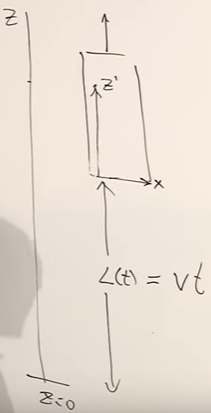
\includegraphics{gr-1-elevator}
\end{figure}

In this lecture we'll ignore Special Relativity, which is tantamount to setting $c=\infty$, or assuming all velocities very small. If General Relativity is the generalization of Special Relativity, how did Einstein get away with ignoring Special Relativity? The answer is that Special Relativity is about high velocities. Gravity has to do with heavy masses. There are situation where the mass is high, but the velocity isn't. Einstein started thinking about these situations, and then combined it with Special relativity to think about the combination of high masses and high velocities.

Let's think about inertial reference frames. If $z$ and $x^\prime$ are inertial, they are related by uniform velocity, so we nave the coordinate transformation:

\begin{align*}
	L(t)=&vt\\
	z^\prime =& z-L(t)\\
	=& z-vt\\
	t^\prime =& t\\
	x^\prime =& x
\end{align*}

Now introduce Newton's 2nd law of motion. How does this change under the coordinate transformation?

\begin{align*}
	F =& m \ddot{z} \text{ in the $z$ frame}\\
	\ddot{z^\prime} =& \ddot{z} \text{ since $v$ is constant, whence:}\\
	F =& m \ddot{z^\prime} \text{ since $v$ is constant, so Newton's 2nd Law holds.}
\end{align*}

Now let's go to an accelerated frame--Figure \ref{fig:gr-1-elevator-accelerated}.

\begin{figure}[H]
	\caption{Elevator in a accelerated Frame}\label{fig:gr-1-elevator-accelerated}
	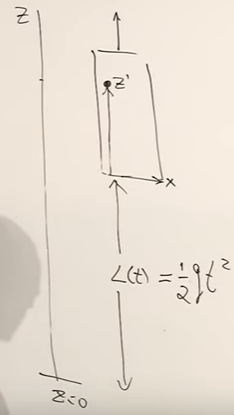
\includegraphics{gr-1-elevator-accelerated}
\end{figure}

The coordinate transformation is now:
\begin{align*}
	L(t)=&vt\\
	z^\prime =& z-\frac{1}{2}g t^2\\
	=& z-vt\\
	t^\prime =& t\\
	x^\prime =& x
\end{align*}

We will continue to assume that Newton's laws hold in the $z$ frame of reference.
\begin{align*}
	\ddot{z^\prime} =& \ddot{z}-g\\
	\underbrace{F -mg}_\text{Force, including fictitious term} =& m \ddot{z^\prime} 
\end{align*}

The fictitious force looks like a uniform gravitational field. The special property of gravity is that gravitational forces are proportional to mass. That has a deep implication: the mass cancels, so the motion doesn't depend on the mass. Most people before Einstein considered this largely an accident. People know that acceleration mimicked gravity; Einstein said it was deep principle of nature. Figure \ref{fig:gr-1-coordinates-const} shows the coordinate transformation for constant velocity. Straight lines go to straight lines. Figure \ref{fig:gr-1-coordinates-accelerated} shows the results of accelerating the coordinate system: straight lines are not preserved. We have a curvy linear transformation. Einstein understood very early that there is a connection between gravity and curvy linear transformations of spacetime. Special Relativity was all about linear transformations

\begin{figure}[H]
	\caption[Coordinate Transformation for constant velocity]{Coordinate Transformation for constant velocity. Green represents constant $z^\prime$}\label{fig:gr-1-coordinates-const}
	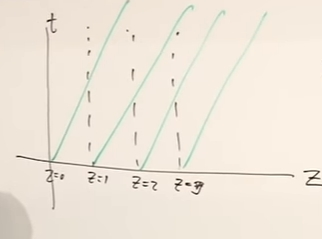
\includegraphics{gr-1-coordinates-const}
\end{figure}

\begin{figure}[H]
	\caption{Coordinate Transformation accelerated}\label{fig:gr-1-coordinates-accelerated}
	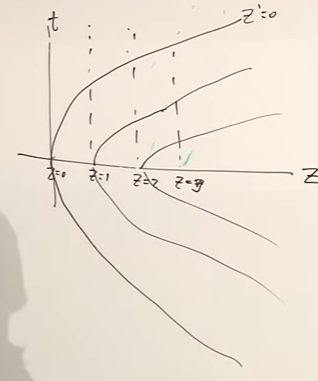
\includegraphics{gr-1-coordinates-accelerated}
\end{figure}

\subsubsection{Example: what is the influence of gravity on light?}
In 1907 most physicists would have thought there was no effect. Einstein argued from the equivalence principle that grapity would affect light. Consider a beam of light in our elevator--Figure \ref{fig:gr-1-elevator-accelerated}.

\begin{figure}[H]
	\caption{What is the influence of gravity on light? }
	\begin{subfigure}[t]{0.5\textwidth}
		\caption{Path of Light in $z$ system}\label{fig:gr-1-light-in-elevator}
		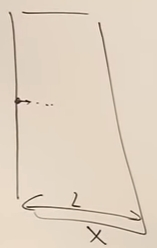
\includegraphics{gr-1-light-in-elevator}
	\end{subfigure}
	\begin{subfigure}[t]{0.5\textwidth}
		\caption{Path of Light in $z^\prime$ system}\label{fig:gr-1-elevator-accelerated-curved-path}
		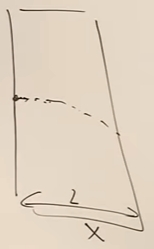
\includegraphics{gr-1-elevator-accelerated-curved-path}
	\end{subfigure}
\end{figure}

We'll write down the equation for the path of the light beam:
\begin{align*}
	x =& ct \text{ in the $z$ frame}\\
	z =& 0 \text{, but in the moving frams}\\
	z^\prime + g\frac{t^2}{2} =&0 \text{, which is curved--Figure \ref{fig:gr-1-elevator-accelerated-curved-path}}
\end{align*}

\begin{itemize}
	\item In the primed system light is bending down;
	\item In the unprimed system the elevator is accelerating--the beam only \emph{looks} curved.
\end{itemize}

Einstein said that they are both the same thing.

What we have learned. 

\begin{enumerate}
	\item It is interesting to think about curvy linear transformations. 
	\item When you think about curvy linear transformations the form of Newton's Laws changes.
	\item One thing that happens is that apparent  gravitational fields  materialize that are apparently indistinguishable from ordinary gravitational fields.
\end{enumerate}

But are they really indistinguishable? Not really. Let's t1lk about gravitational fields generated by the Sun or the Earth--Figure \ref{fig:gr-1-suns-gravitational-field}. It is pretty obvious that there is no way to do a coordinate transformation like the ones we've been discussing which will remove the gravitational field. In \ref{fig:gr-1-suns-gravitational-field-local} we are in a laboratory we can transform away the field locally,  but there is no way to get rid of the fact that we are dealing with a filed that is inwards globally.

\begin{figure}[H]
	\caption{Sun's Gravitational Field}
	\begin{subfigure}[t]{0.5\textwidth}
		\caption{There is no way to do a coordinate transformation like the ones we've been discussing which will remove the gravitational field}\label{fig:gr-1-suns-gravitational-field}
		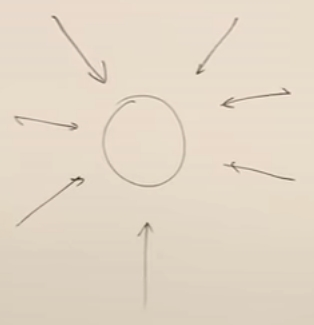
\includegraphics[width=\textwidth]{gr-1-suns-gravitational-field}
	\end{subfigure}
	\begin{subfigure}[t]{0.5\textwidth}
		\caption{If we are in a laboratory we can transform away the field locally, but there is no way to get rid of the fact that we are dealing with a filed that is inwards globally.}\label{fig:gr-1-suns-gravitational-field-local}
		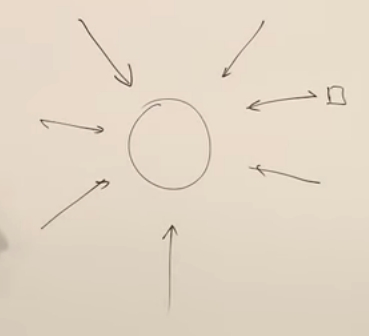
\includegraphics[width=\textwidth]{gr-1-suns-gravitational-field-local}
	\end{subfigure}
\end{figure}

Figure \ref{fig:2000:mile:man} shows why we can't transform the field away. In Figure \ref{fig:gr-1-suns-gravitational-field-2000-mile-ff} is oriented with his feet towards the Sun: fe feels a tidal pull, as his feet are closer to the Sun than his head. In Figure \ref{fig:gr-1-suns-gravitational-field-2000-mile} he feels pressure at his head and feet. Being squashed is not something we can get rid of by performing a coordinate transformation. So it is not true that gravity is equivalent to a coordinate transformation. Einstein said that for small objects and small times, gravity was equivalent to a coordinate transformation.
\begin{figure}[H]
	\caption{2000 mile man}\label{fig:2000:mile:man}
		\begin{subfigure}[t]{0.5\textwidth}
		\caption{If we are in a laboratory we can transform away the field locally, but there is no way to get rid of the fact that we are dealing with a filed that is inwards globally.}\label{fig:gr-1-suns-gravitational-field-2000-mile-ff}
		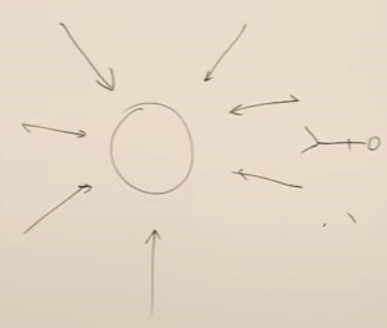
\includegraphics[width=\textwidth]{gr-1-suns-gravitational-field-2000-mile-ff}
	\end{subfigure}
	\begin{subfigure}[t]{0.5\textwidth}
		\caption{If we are in a laboratory we can transform away the field locally, but there is no way to get rid of the fact that we are dealing with a filed that is inwards globally.}\label{fig:gr-1-suns-gravitational-field-2000-mile}
		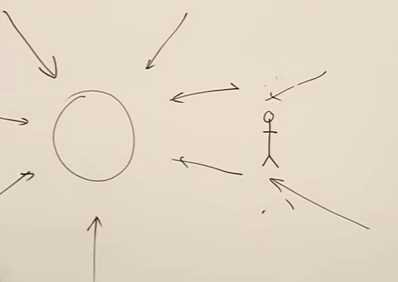
\includegraphics[width=\textwidth]{gr-1-suns-gravitational-field-2000-mile}
	\end{subfigure}
\end{figure}

That raises a question: if I present you with a force field, e.g. the force field of uniform acceleration--Figure \ref{fig:gr-1-uniform-force-field}--you can make it look more complicated via a suitable transformation. If transformation involve the $x$ axis it can make the field bend. Or accelerate along $z$ while oscillating along $x$. This will give a complicated apparent gravitational field. If I tell you what the field is everywhere, how do I determine if it is just a fake gravitational field, from acceleration, or a real genuine one? If it is Newtonian gravitational field, just calculate the tidal forces on a freely falling object. If there is squeezing or stretching we have gravity,  otherwise not. If you can transform the field away it is not real gravity, otherwise it is real (can detect tidal forces via crystal).

\begin{figure}[H]
	\caption{Uniform Force Field}\label{fig:gr-1-uniform-force-field}
	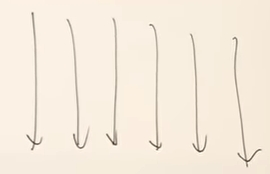
\includegraphics{gr-1-uniform-force-field}
\end{figure}


Einstein asked what kind of mathematics he needed to answer the questions about real and apparent gravitational fields. The other element was special relativity: he know from the work of Minkowski that special relativity had a geometry associated with it, which had a length, proper distance.

\begin{align*}
	d\tau^2 =& dt^2 - dx^2 \text{, or, depending on who you are}\\
	ds^2 =& dx^2 -dt^2
\end{align*}

Einstein realized that the problem of deciding whether or not a gravitation filed was real was similar to a problem that Riemann had explored, deciding whether or not a space was flat. Riemann had not considered metrics with a minus sign. In Euclidean space:
\begin{align*}
	ds^2 =& \sum (dx^i)^2 \numberthis \label{eq:euclidean:metric}
\end{align*}
 
Gauss had already understood that in non-Euclidean spaces the formula for distance on a surface was more complicated. Riemann took the next step. Consider a curved surface (let's not worry what this means exactly), and lay out coordinates as in Figure \ref{fig:gr-1-curved-surface-coordinates}.
 
\begin{figure}[H]
	\caption[Curved Surface with coordinates]{Curved Surface with coordinates. Don't worry about straight lines.}\label{fig:gr-1-curved-surface-coordinates}
	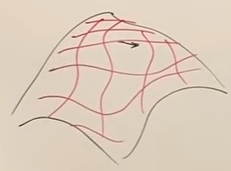
\includegraphics{gr-1-curved-surface-coordinates}
\end{figure} 

The formula for the distance between two close points becomes:
\begin{align*}
	ds^2 =& \sum_{m,n} g_{mn}(x) dx^m dx^n
\end{align*}
It works also for curved coordinates in a flat space.

We are building up geometry in little regions and piecing them together. Maybe we can put them together on a flat plane, but maybe not. So, given the little pieces, how do we know whether or not it is flat? Is there a coordinate system where (\ref{eq:euclidean:metric}) holds?

We have two parallel questions. Can we find a coordinate system:
\begin{itemize}
	\item where apparent gravitational field is zero;
	\item where (\ref{eq:euclidean:metric}) is true.
\end{itemize}

We will need the mathematics of Tensor Analysis.

\subsection{Tensor Analysis}

Can we change $g_{mn}$ to $\delta_{mn}$? First question is how does $g_{mn}$ change when we change coordinates?

We have two sets of coordinates, $x$ and $y$, and write $x^m = x^m(y)$, and $y^m = y^m(x)$. How do $dx_m$ transform?

\begin{align*}
	dy^m =& \sum_p \frac{\partial y^m}{\partial x^p} dx^p\\
	V^{\prime m} =& \sum_p \frac{\partial y^m}{\partial x^p} V^p \text{, or, using Einstein's summation convention} \\
	V^{\prime m} =&  \frac{\partial y^m}{\partial x^p} V^p \numberthis \label{eq:contravariant}
\end{align*}

\begin{defn}[Contravariant]
	A Vector whose components transform in accordance with (\ref{eq:contravariant}) is said to be \emph{contravariant}.
\end{defn}

Consider a scalar function, $s$, then the gradient is a vector.

\begin{defn}[Gradient]
	The gradient of $s$ is $\frac{\partial s}{\partial x^p}$.
\end{defn}

\begin{align*}
	\frac{\partial s}{\partial y^m} =& \frac{\partial s}{\partial x^p}\frac{\partial x^p}{\partial y^m}\\
	W_m^\prime =& \frac{\partial x^p}{\partial y^m} W_p \numberthis \label{eq:covariant}
\end{align*}

\begin{defn}[Covariant]
	A Vector whose components transform in accordance with (\ref{eq:covariant}) is said to be \emph{covariant}.
\end{defn}
 
Relativity is about the transformation properties of objects.

To define more general tensors, consider products of vectors -- e.g.
\begin{align*}
	V^mU^n=&T^{mn} \text{, contravariant tensor of rank 2 }
\end{align*}

LS derived the transformation properties, and showed that $g_mn$ is covariant.


\section{Tensor mathematics}

A good notation will carry you a long way. When it is good it tells you what to do next. It's like tinker toys: you put the stick into a hole. The notation of GR is like that: if you follow the rules it is difficult to make mistakes. The rules are tensor analysis and tensor algebra.

\subsection{Flat space}

Our aim is to distinguish flat from not flat. LS rolls flat page into cylinder, which is locally flat (it has extrinsic curvature from the embedding in 3D, not intrinsic: a tiny bug embedded in the surface can't notice this sort of curvature, but can find intrinsic curvature). Riemannian geometry is about intrinsic properties of space.
 
Figures \ref{fig:gr-2-lattice} and \ref{fig:gr-2-lattice-not-flat} illustrate a surface can be flattened and one that cannot. A curved surface is one that cannot be flattened without distorting it.

\begin{figure}[H]
	\caption{Can we flatten the lattice onto a surface?}
	\begin{subfigure}[t]{0.5\textwidth}
		\caption{Flat Lattice of equilateral triangles. These can be drawn on a plane.}\label{fig:gr-2-lattice}
		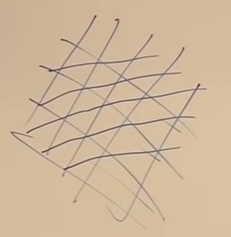
\includegraphics[width=\textwidth]{gr-2-lattice}
	\end{subfigure}
	\begin{subfigure}[t]{0.5\textwidth}
		\caption{Not a Flat Lattice: the bold lines are twice the length of the others, so the central one is forced up, out of blackboard.}\label{fig:gr-2-lattice-not-flat}
		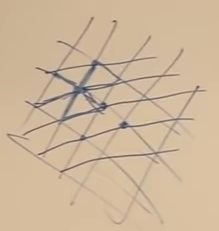
\includegraphics[width=\textwidth]{gr-2-lattice-not-flat}
	\end{subfigure}
\end{figure}

Our problem is to decide whether or not a space is really flat. What are we given? We are given a metric tensor.

\subsection{Metric tensor}

\subsection{Scalars transform trivially}

\begin{align*}
	x^m \leftrightarrow& y^m \\
	S^\prime(y) =& S(x) \text{, we call such an $s$ a scalar}
\end{align*}

Figure \ref{fig:gr-2-coordinates} depicts a coordinate system, and a vector $\vec{V}$.
\begin{figure}[H]
	\caption[A set of coordinates, not necessarily perpendicular.]{A set of coordinates, not necessarily perpendicular (although they could be). Furthermore the distances along the axes are just labels: they need not be equidistant. There are two unit vectors, $\vec{e_1}$ and $\vec{e_2}$ along the $x_1$ and $x_2$ axes.}\label{fig:gr-2-coordinates}
	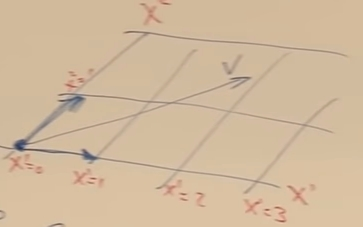
\includegraphics{gr-2-coordinates}
\end{figure}

$\vec{V}$ can be expanded:
\begin{align*}
	\vec{V} =& \sum_i V^i \vec{e_i} \numberthis \label{eq:contravariant:components}
\end{align*}

\begin{defn}[Contravariant components]
	 In (\ref{eq:contravariant:components}), the numbers $V^i$ are called the\emph{ contravariant components} of $\vec{V}$.
\end{defn}

\url{https://youtu.be/5VKyRVLMMQ4?t=1230}

\subsection{Scalar and tensor fields}
\subsection{Tensor analysis}
\subsection{Tensor mathematics: addition, multiplication, contraction}

\section{Flatness \& curvature}

TBP

\section{Geodesics \& gravity}

TBP

\section{Metric for a gravitational field}

TBP

\section{Black holes}

TBP

\section{Falling into a black hole}

TBP

\section{Formation of a black hole}

TBP

\section{Einstein field equations}

TBP

\section{Gravity Waves}

TBP

\bibliographystyle{unsrt}
\addcontentsline{toc}{section}{Bibliography}
\raggedright
\bibliography{tm}

\end{document}
